% This file was created by tikzplotlib v0.9.1.
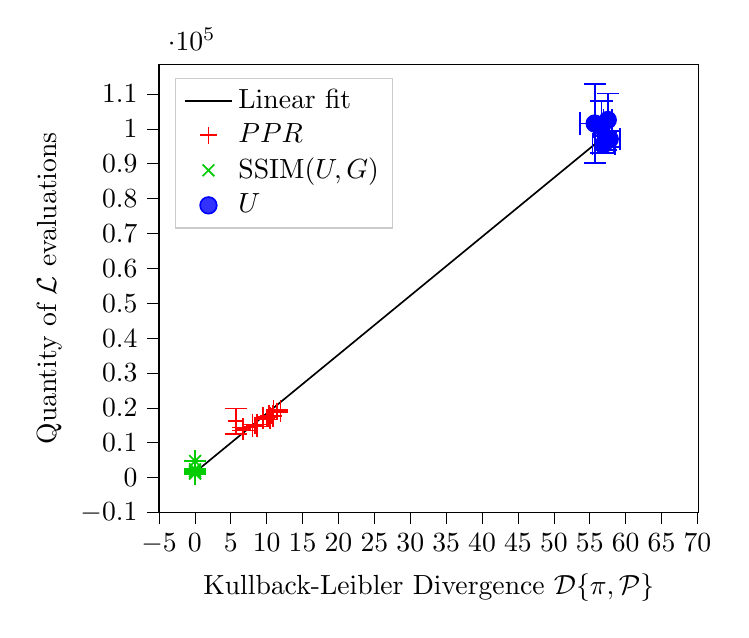
\begin{tikzpicture}

\definecolor{color0}{rgb}{1,0.0,0.0}
\definecolor{color1}{rgb}{0,0.8,0.0}
\definecolor{color2}{rgb}{0.0,0.0,1}
\definecolor{color3}{rgb}{0.0,0.0,0.0}

\begin{axis}[
legend cell align={left},
legend style={fill opacity=0.8, draw opacity=1, text opacity=1, at={(0.03,0.97)}, anchor=north west, draw=white!80!black},
tick align=outside,
tick pos=left,
x grid style={white!69.0196078431373!black},
xlabel={Kullback-Leibler Divergence \(\displaystyle {\cal D} \{\pi, {\cal P}\}\)},
xmin=-5.0, xmax=70.1613818701095,
xtick style={color=black},
xtick distance=5,
ytick distance=10000,
y grid style={white!69.0196078431373!black},
ylabel={Quantity of \({\cal L}\) evaluations},
ymin=-10000.00, ymax=118545.85,
ytick style={color=black}
]
\path [draw=color0, semithick]
(axis cs:5.71795365099151,16157.5)
--(axis cs:5.77133948534581,16157.5);

\path [draw=color0, semithick]
(axis cs:6.6768824419002,13953)
--(axis cs:6.77321107556694,13953);

\path [draw=color0, semithick]
(axis cs:8.02877279045042,14940.5)
--(axis cs:8.63543918622054,14940.5);

\path [draw=color0, semithick]
(axis cs:9.52185212376919,17043)
--(axis cs:10.4908349952443,17043);

\path [draw=color0, semithick]
(axis cs:10.3029683750536,17720.5)
--(axis cs:10.9155451202318,17720.5);

\path [draw=color0, semithick]
(axis cs:10.954510866509,19064.5)
--(axis cs:11.9335782130671,19064.5);

\path [draw=color0, semithick]
(axis cs:5.74464656816866,12446)
--(axis cs:5.74464656816866,19869);

\path [draw=color0, semithick]
(axis cs:6.72504675873357,13488)
--(axis cs:6.72504675873357,14418);

\path [draw=color0, semithick]
(axis cs:8.33210598833548,14689)
--(axis cs:8.33210598833548,15192);

\path [draw=color0, semithick]
(axis cs:10.0063435595067,16676)
--(axis cs:10.0063435595067,17410);

\path [draw=color0, semithick]
(axis cs:10.6092567476427,17618)
--(axis cs:10.6092567476427,17823);

\path [draw=color0, semithick]
(axis cs:11.4440445397881,18822)
--(axis cs:11.4440445397881,19307);

\path [draw=color1, semithick]
(axis cs:0.0271909650803472,2382.5)
--(axis cs:0.030089733601838,2382.5);

\path [draw=color1, semithick]
(axis cs:0.029683008672791,1207.5)
--(axis cs:0.0308036500189849,1207.5);

\path [draw=color1, semithick]
(axis cs:0.0282101242046804,1738.5)
--(axis cs:0.0298855157628486,1738.5);

\path [draw=color1, semithick]
(axis cs:0.0278177027329167,4757)
--(axis cs:0.0348526563256524,4757);

\path [draw=color1, semithick]
(axis cs:0.0232802581598788,1829.5)
--(axis cs:0.0301604324600733,1829.5);

\path [draw=color1, semithick]
(axis cs:0.0304771056975755,1224)
--(axis cs:0.0323746358923458,1224);

\path [draw=color1, semithick]
(axis cs:0.0286403493410926,2120)
--(axis cs:0.0286403493410926,2645);

\path [draw=color1, semithick]
(axis cs:0.0302433293458879,1163)
--(axis cs:0.0302433293458879,1252);

\path [draw=color1, semithick]
(axis cs:0.0290478199837645,1565)
--(axis cs:0.0290478199837645,1912);

\path [draw=color1, semithick]
(axis cs:0.0313351795292845,4698)
--(axis cs:0.0313351795292845,4816);

\path [draw=color1, semithick]
(axis cs:0.026720345309976,1740)
--(axis cs:0.026720345309976,1919);

\path [draw=color1, semithick]
(axis cs:0.0314258707949607,1138)
--(axis cs:0.0314258707949607,1310);

\path [draw=color2, semithick]
(axis cs:53.6407046096139,101541)
--(axis cs:57.7293889288474,101541);

\path [draw=color2, semithick]
(axis cs:56.1280894679801,96497)
--(axis cs:58.3022565457241,96497);

\path [draw=color2, semithick]
(axis cs:55.3633380690649,95565)
--(axis cs:58.47445725549,95565);

\path [draw=color2, semithick]
(axis cs:55.5223746731559,100523.5)
--(axis cs:57.7271641567295,100523.5);

\path [draw=color2, semithick]
(axis cs:56.8924880373743,102562.5)
--(axis cs:58.1261131182599,102562.5);

\path [draw=color2, semithick]
(axis cs:56.3603430284318,97066.5)
--(axis cs:59.2024246504929,97066.5);

\path [draw=color2, semithick]
(axis cs:55.6850467692306,90127)
--(axis cs:55.6850467692306,112955);

\path [draw=color2, semithick]
(axis cs:57.2151730068521,94020)
--(axis cs:57.2151730068521,98974);

\path [draw=color2, semithick]
(axis cs:56.9188976622774,93149)
--(axis cs:56.9188976622774,97981);

\path [draw=color2, semithick]
(axis cs:56.6247694149427,93079)
--(axis cs:56.6247694149427,107968);

\path [draw=color2, semithick]
(axis cs:57.5093005778171,94974)
--(axis cs:57.5093005778171,110151);

\path [draw=color2, semithick]
(axis cs:57.7813838394624,94657)
--(axis cs:57.7813838394624,99476);

\addplot [semithick, color0, mark=|, mark size=4, mark options={solid}, only marks, forget plot]
table {%
5.71795365099151 16157.5
6.6768824419002 13953
8.02877279045042 14940.5
9.52185212376919 17043
10.3029683750536 17720.5
10.954510866509 19064.5
};
\addplot [semithick, color0, mark=|, mark size=4, mark options={solid}, only marks, forget plot]
table {%
5.77133948534581 16157.5
6.77321107556694 13953
8.63543918622054 14940.5
10.4908349952443 17043
10.9155451202318 17720.5
11.9335782130671 19064.5
};
\addplot [semithick, color0, mark=-, mark size=4, mark options={solid}, only marks, forget plot]
table {%
5.74464656816866 12446
6.72504675873357 13488
8.33210598833548 14689
10.0063435595067 16676
10.6092567476427 17618
11.4440445397881 18822
};
\addplot [semithick, color0, mark=-, mark size=4, mark options={solid}, only marks, forget plot]
table {%
5.74464656816866 19869
6.72504675873357 14418
8.33210598833548 15192
10.0063435595067 17410
10.6092567476427 17823
11.4440445397881 19307
};
\addplot [semithick, color1, mark=|, mark size=4, mark options={solid}, only marks, forget plot]
table {%
0.0271909650803472 2382.5
0.029683008672791 1207.5
0.0282101242046804 1738.5
0.0278177027329167 4757
0.0232802581598788 1829.5
0.0304771056975755 1224
};
\addplot [semithick, color1, mark=|, mark size=4, mark options={solid}, only marks, forget plot]
table {%
0.030089733601838 2382.5
0.0308036500189849 1207.5
0.0298855157628486 1738.5
0.0348526563256524 4757
0.0301604324600733 1829.5
0.0323746358923458 1224
};
\addplot [semithick, color1, mark=-, mark size=4, mark options={solid}, only marks, forget plot]
table {%
0.0286403493410926 2120
0.0302433293458879 1163
0.0290478199837645 1565
0.0313351795292845 4698
0.026720345309976 1740
0.0314258707949607 1138
};
\addplot [semithick, color1, mark=-, mark size=4, mark options={solid}, only marks, forget plot]
table {%
0.0286403493410926 2645
0.0302433293458879 1252
0.0290478199837645 1912
0.0313351795292845 4816
0.026720345309976 1919
0.0314258707949607 1310
};
\addplot [semithick, color2, mark=|, mark size=4, mark options={solid}, only marks, forget plot]
table {%
53.6407046096139 101541
56.1280894679801 96497
55.3633380690649 95565
55.5223746731559 100523.5
56.8924880373743 102562.5
56.3603430284318 97066.5
};
\addplot [semithick, color2, mark=|, mark size=4, mark options={solid}, only marks, forget plot]
table {%
57.7293889288474 101541
58.3022565457241 96497
58.47445725549 95565
57.7271641567295 100523.5
58.1261131182599 102562.5
59.2024246504929 97066.5
};
\addplot [semithick, color2, mark=-, mark size=4, mark options={solid}, only marks, forget plot]
table {%
55.6850467692306 90127
57.2151730068521 94020
56.9188976622774 93149
56.6247694149427 93079
57.5093005778171 94974
57.7813838394624 94657
};
\addplot [semithick, color2, mark=-, mark size=4, mark options={solid}, only marks, forget plot]
table {%
55.6850467692306 112955
57.2151730068521 98974
56.9188976622774 97981
56.6247694149427 107968
57.5093005778171 110151
57.7813838394624 99476
};
\addplot [semithick, color3]
table {%
0.026720345309976 1539.88164299791
0.610100784644849 2525.39064984014
1.19348122397972 3510.89965668237
1.77686166331459 4496.4086635246
2.36024210264947 5481.91767036683
2.94362254198434 6467.42667720906
3.52700298131921 7452.93568405129
4.11038342065408 8438.44469089352
4.69376385998896 9423.95369773575
5.27714429932383 10409.462704578
5.8605247386587 11394.9717114202
6.44390517799357 12380.4807182624
7.02728561732845 13365.9897251047
7.61066605666332 14351.4987319469
8.19404649599819 15337.0077387891
8.77742693533306 16322.5167456314
9.36080737466794 17308.0257524736
9.94418781400281 18293.5347593158
10.5275682533377 19279.043766158
11.1109486926726 20264.5527730003
11.6943291320074 21250.0617798425
12.2777095713423 22235.5707866847
12.8610900106772 23221.079793527
13.444470450012 24206.5888003692
14.0278508893469 25192.0978072114
14.6112313286818 26177.6068140537
15.1946117680167 27163.1158208959
15.7779922073515 28148.6248277381
16.3613726466864 29134.1338345803
16.9447530860213 30119.6428414226
17.5281335253562 31105.1518482648
18.111513964691 32090.660855107
18.6948944040259 33076.1698619493
19.2782748433608 34061.6788687915
19.8616552826956 35047.1878756337
20.4450357220305 36032.6968824759
21.0284161613654 37018.2058893182
21.6117966007003 38003.7148961604
22.1951770400351 38989.2239030026
22.77855747937 39974.7329098449
23.3619379187049 40960.2419166871
23.9453183580397 41945.7509235293
24.5286987973746 42931.2599303716
25.1120792367095 43916.7689372138
25.6954596760444 44902.277944056
26.2788401153792 45887.7869508982
26.8622205547141 46873.2959577405
27.445600994049 47858.8049645827
28.0289814333839 48844.3139714249
28.6123618727187 49829.8229782672
29.1957423120536 50815.3319851094
29.7791227513885 51800.8409919516
30.3625031907233 52786.3499987938
30.9458836300582 53771.8590056361
31.5292640693931 54757.3680124783
32.112644508728 55742.8770193205
32.6960249480628 56728.3860261628
33.2794053873977 57713.895033005
33.8627858267326 58699.4040398472
34.4461662660675 59684.9130466895
35.0295467054023 60670.4220535317
35.6129271447372 61655.9310603739
36.1963075840721 62641.4400672161
36.7796880234069 63626.9490740584
37.3630684627418 64612.4580809006
37.9464489020767 65597.9670877428
38.5298293414116 66583.4760945851
39.1132097807464 67568.9851014273
39.6965902200813 68554.4941082695
40.2799706594162 69540.0031151118
40.863351098751 70525.512121954
41.4467315380859 71511.0211287962
42.0301119774208 72496.5301356384
42.6134924167557 73482.0391424807
43.1968728560905 74467.5481493229
43.7802532954254 75453.0571561651
44.3636337347603 76438.5661630074
44.9470141740952 77424.0751698496
45.53039461343 78409.5841766918
46.1137750527649 79395.093183534
46.6971554920998 80380.6021903763
47.2805359314346 81366.1111972185
47.8639163707695 82351.6202040607
48.4472968101044 83337.129210903
49.0306772494393 84322.6382177452
49.6140576887741 85308.1472245874
50.197438128109 86293.6562314297
50.7808185674439 87279.1652382719
51.3641990067788 88264.6742451141
51.9475794461136 89250.1832519564
52.5309598854485 90235.6922587986
53.1143403247834 91221.2012656408
53.6977207641182 92206.710272483
54.2811012034531 93192.2192793253
54.864481642788 94177.7282861675
55.4478620821229 95163.2372930097
56.0312425214577 96148.746299852
56.6146229607926 97134.2553066942
57.1980034001275 98119.7643135364
57.7813838394624 99105.2733203786
};
\addlegendentry{Linear fit}
\addplot [semithick, color0, mark=+, mark size=3, mark options={solid}, only marks]
table {%
5.74464656816866 16157.5
6.72504675873357 13953
8.33210598833548 14940.5
10.0063435595067 17043
10.6092567476427 17720.5
11.4440445397881 19064.5
};
\addlegendentry{$PPR$}
\addplot [semithick, color1, mark=x, mark size=3, mark options={solid}, only marks]
table {%
0.0286403493410926 2382.5
0.0302433293458879 1207.5
0.0290478199837645 1738.5
0.0313351795292845 4757
0.026720345309976 1829.5
0.0314258707949607 1224
};
\addlegendentry{SSIM$(U,G)$}
\addplot [semithick, color2, mark=*, mark size=3, mark options={solid}, only marks]
table {%
55.6850467692306 101541
57.2151730068521 96497
56.9188976622774 95565
56.6247694149427 100523.5
57.5093005778171 102562.5
57.7813838394624 97066.5
};
\addlegendentry{$U$}
\end{axis}

\end{tikzpicture}
